\begin{exercício}{Momento de dipolo de uma esfera carregada com cavidade}{exercício4}
    Considere um objeto esférico maciço de raio \(a\) contendo uma cavidade de raio \(b\), localizada a uma distância \(d\) de seu centro, como mostra a figura abaixo.
    \begin{center}
        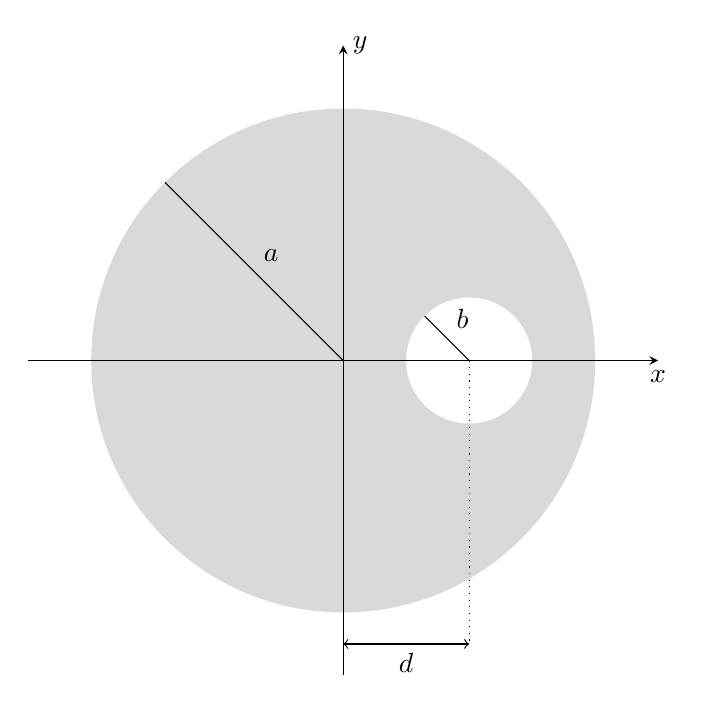
\begin{tikzpicture}[scale=0.8]
        % Shaded circles
        \fill[gray!30] (0,0) circle (4cm);  % Outer shaded region
        \fill[white] (2,0) circle (1cm);  % Inner white circle

        % Axes
        \draw[-stealth] (-5,0) -- (5,0) node[anchor=north] {\(x\)}; % x-axis
        \draw[-stealth] (0,-5) -- (0,5) node[anchor=west] {\(y\)};  % y-axis

        % Outer radius
        \draw (0,0) -- ({4*cos(135)},{4*sin(135)}) node[midway, above, anchor=south west] {\(a\)};  % Outer radius

        % Inner radius
        \draw (2,0) -- ({2 + 1*cos(135)},{1*sin(135)}) node[midway, above, anchor=south west] {\(b\)};  % Inner radius

        % Distance label (d)
        \draw[<->] (0,-4.5) -- (2,-4.5) node[midway, anchor=north] {\(d\)};
        \draw[dotted] (2,0) -- (2,-4.5);
    \end{tikzpicture}
    \end{center}
    A região hachurada do objeto está carregada com uma densidade volumétrica de carga uniforme \(\rho\), enquanto não há cargas dentro da cavidade. Utilizando o sistema de coordenadas mostrado na figura, com a origem sobre o centro do objeto, calcule o momento de dipolo \(\vetor{p}\) do sistema. Refaça a conta agora colocando a origem do sistema de coordenadas sobre o centro da cavidade. Determine um sistema de coordenadas sob o qual o momento de dipolo é o vetor nulo.
\end{exercício}
\begin{proof}[Resolução]

\end{proof}
